\section{ЗАДАНИЕ}

Используя хвостовую рекурсию, разработать эффективную программу, (комментируя назначение аргументов), позволяющую:

\begin{enumerate}
    \item Найти длину списка (по верхнему уровню);
    \item Найти сумму элементов числового списка;
    \item Найти сумму элементов числового списка, стоящих на нечетных позициях исходного списка (нумерация от 0).
\end{enumerate}

\begin{lstlisting}[caption=Текст программы]
domains
	list = integer*.
	index = integer.

predicates
	length(list, integer).
	sum(list, integer).
	sumOdd(list, integer).
	sumOdd(list, integer, index).

clauses
	length([], 0) :- !.
	length([_|Tail], Length) :-
		length(Tail, TailLength),
		Length = TailLength + 1.

	sum([], 0) :- !.
	sum([Head|Tail], Sum) :-
		sum(Tail, TailSum),
		Sum = TailSum + Head.

	sumOdd(List, Sum) :- sumOdd(List, Sum, 0).
	sumOdd([], 0, _) :- !.
	sumOdd([_|Tail], Sum, Index) :-
		Index mod 2 = 0,
		NextIndex = Index + 1,
		sumOdd(Tail, Sum, NextIndex).
	sumOdd([Head|Tail], Sum, Index) :-
		Index mod 2 = 1,
		NextIndex = Index + 1,
		sumOdd(Tail, TailSum, NextIndex),
		Sum = TailSum + Head.

goal
	length([1, 2, 3, 4, 5], Length);
	sum([1, 2, 3, 4, 5, 6], Sum);
	sumOdd([1, 2, 1, 2, 1, 2], SumOdd).
\end{lstlisting}

\section{РЕЗУЛЬТАТ РАБОТЫ}

\begin{figure}[H]
    \centering
    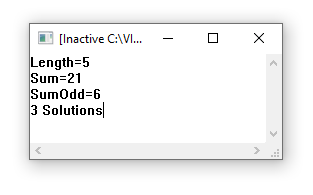
\includegraphics{img/result.png}
    \caption{Результат работы программы}
\end{figure}
